%--------------------------% 
% PREAMBLE 1 - DO NOT EDIT %
%--------------------------% 
%%%%%%%%%%%%%%%%%%%%%%%%
% PREAMBLE %%%%%%%%%%%%%
%%%%%%%%%%%%%%%%%%%%%%%%

\expandafter\gdef\csname ver@amssymb.sty\endcsname{9999/12/31}
\expandafter\gdef\csname ver@amsfonts.sty\endcsname{9999/12/31}

\documentclass[12pt,twoside]{article}

\global\expandafter\let\csname ver@amssymb.sty\endcsname\relax
\global\expandafter\let\csname ver@amsfonts.sty\endcsname\relax

\usepackage[small,bf]{caption}
\usepackage[charter]{mathdesign}
\usepackage{amsmath}
\usepackage{graphicx}
\usepackage{qtree}
\usepackage{subcaption}
\usepackage{fancyhdr}
%\usepackage{amsthm}
\usepackage{float}
\usepackage{pdflscape}
\usepackage[hidelinks]{hyperref}
\usepackage{lipsum}
\usepackage{enumitem}
\setlength{\headheight}{40pt}

\newtheorem{theorem}{Theorem}

% PAGE DIMENSIONS
\voffset=-.5in
\hoffset=-.75in
\oddsidemargin=0.65in
\evensidemargin=0.65in
\topmargin=-0.15in
\textheight=9.1in
\textwidth=6.7in

% COLOUR STUFF
\usepackage[dvipsnames]{xcolor}
\definecolor{acolor}{RGB}{118,32,43} % Colour of the article title and sections
\newcommand*{\newhref}[2]{\href{#1}{\textbf{\textcolor{acolor}{#2}}}}
\newcommand{\localtextbulletone}{\textcolor{acolor}{\raisebox{.45ex}{\rule{.6ex}{.6ex}}}}
\renewcommand{\labelitemi}{\localtextbulletone}

\usepackage{sectsty}
\sectionfont{\color{acolor}}  % sets colour of chapters
\subsectionfont{\color{acolor}}  % sets colour of sections

%\addto{\captionsenglish}{\renewcommand{\abstractname}{Summary}}
\makeatletter
\renewcommand{\maketitle}{\bgroup\setlength{\parindent}{0pt}
\begin{flushleft}
  \textbf{\@title}
  
  \@author
\end{flushleft}\egroup
}
\renewcommand{\footrulewidth}{0.4pt}% default is 0pt
\makeatother

%-----------------------------% 
% PROJECT-SPECIFIC PARAMETERS %
%-----------------------------% 
\newcommand{\thedraft}{(DRAFT)}
%\newcommand{\thedraft}{}

\newcommand{\titlestring}{Construction Incidents on Canadian Pipelines}
\newcommand{\theprojectnumber}{4376E-F19-CER-001}
\newcommand{\theclient}{Ms. Margaret Skwara}
\newcommand{\theshortclient}{Ms. Skwara}
\newcommand{\theclientrole}{Market Analyst \\ Integrated Energy Information and Analysis \\ Canada Energy Regulator}
\newcommand{\theclientaddress}{Suite 210, 517 Tenth Avenue SW \\ Calgary, Alberta T2R 0A8 \\ Canada}
\newcommand{\thestudents}{Smit Patel, Maia Pelletier, Dhruv Pramod, Andrew Willits,\ }
\newcommand{\theshortstudents}{S Patel, M Pelletier, D Pramod, A Willits,\ }

%--------------------------% 
% PREAMBLE 2 - DO NOT EDIT %
%--------------------------%


\title{\textcolor{acolor}{\LARGE{\titlestring}}}

\author{\ \\ \normalsize{\thestudents Patrick Boily} \\ \small{Department of Mathematics and Statistics, University of Ottawa}  \\ \ \\ \today }


\renewcommand{\sectionmark}[1]{\markboth{\textsc{#1}}{}}
\newcommand{\newl}{\newline\newline}

\begin{document}


\begingroup
\let\center\flushleft
\let\endcenter\endflushleft
\maketitle
\thispagestyle{fancy}
\lhead{}
\chead{
\includegraphics[height=35pt]{Images/uOttawa}\hfill 
\includegraphics[height=35pt]{Images/dms}}
\rhead{}
\lfoot{\ }
\cfoot{\footnotesize{STEM Complex, room 541 $-$ 150 Louis-Pasteur Pvt., 
Ottawa, ON, Canada K1N 6N5 $-$ \newhref{mailto:pboily@uottawa.ca}{pboily@uottawa.ca}}}

\endgroup
\small
\tableofcontents
\newpage
\listoffigures
%\newpage
%\listoftables
\normalsize
\newpage\noindent

\pagestyle{fancy}
\lhead[\textsc{Construction Incidents on CDN Pipelines}]{\theshortstudents P Boily}
\rhead[\theshortstudents P Boily]{\leftmark}
\chead{}
\rfoot[\footnotesize\thepage]{\footnotesize{Project Number: \theprojectnumber }}
\cfoot{}
\lfoot[\footnotesize{Project Number: \theprojectnumber }]{\footnotesize{\thepage}}


%-----------------%
% START OF REPORT %
%-----------------%
\section{Project Overview and Statement}
%\begin{figure}[t]
%\centering
%    
\includegraphics[width=0.67\textwidth]{Images/cerlogo.png}
%  \caption[Behold, the logo.]{The Canada Energy Regulator's current logo.}\hrule
%          \label{fig:fig1}
%\end{figure}

A large section of Canada's GDP comes from the oil and natural gas business; therefore, it is important to ensure our gas industry operates safely and ethically. The Canada Energy Regulator (CER) is an agency of the government of Canada designed to moderate all energy-related activities and concerns on a federal level.

\begin{figure}[t]
\centering
    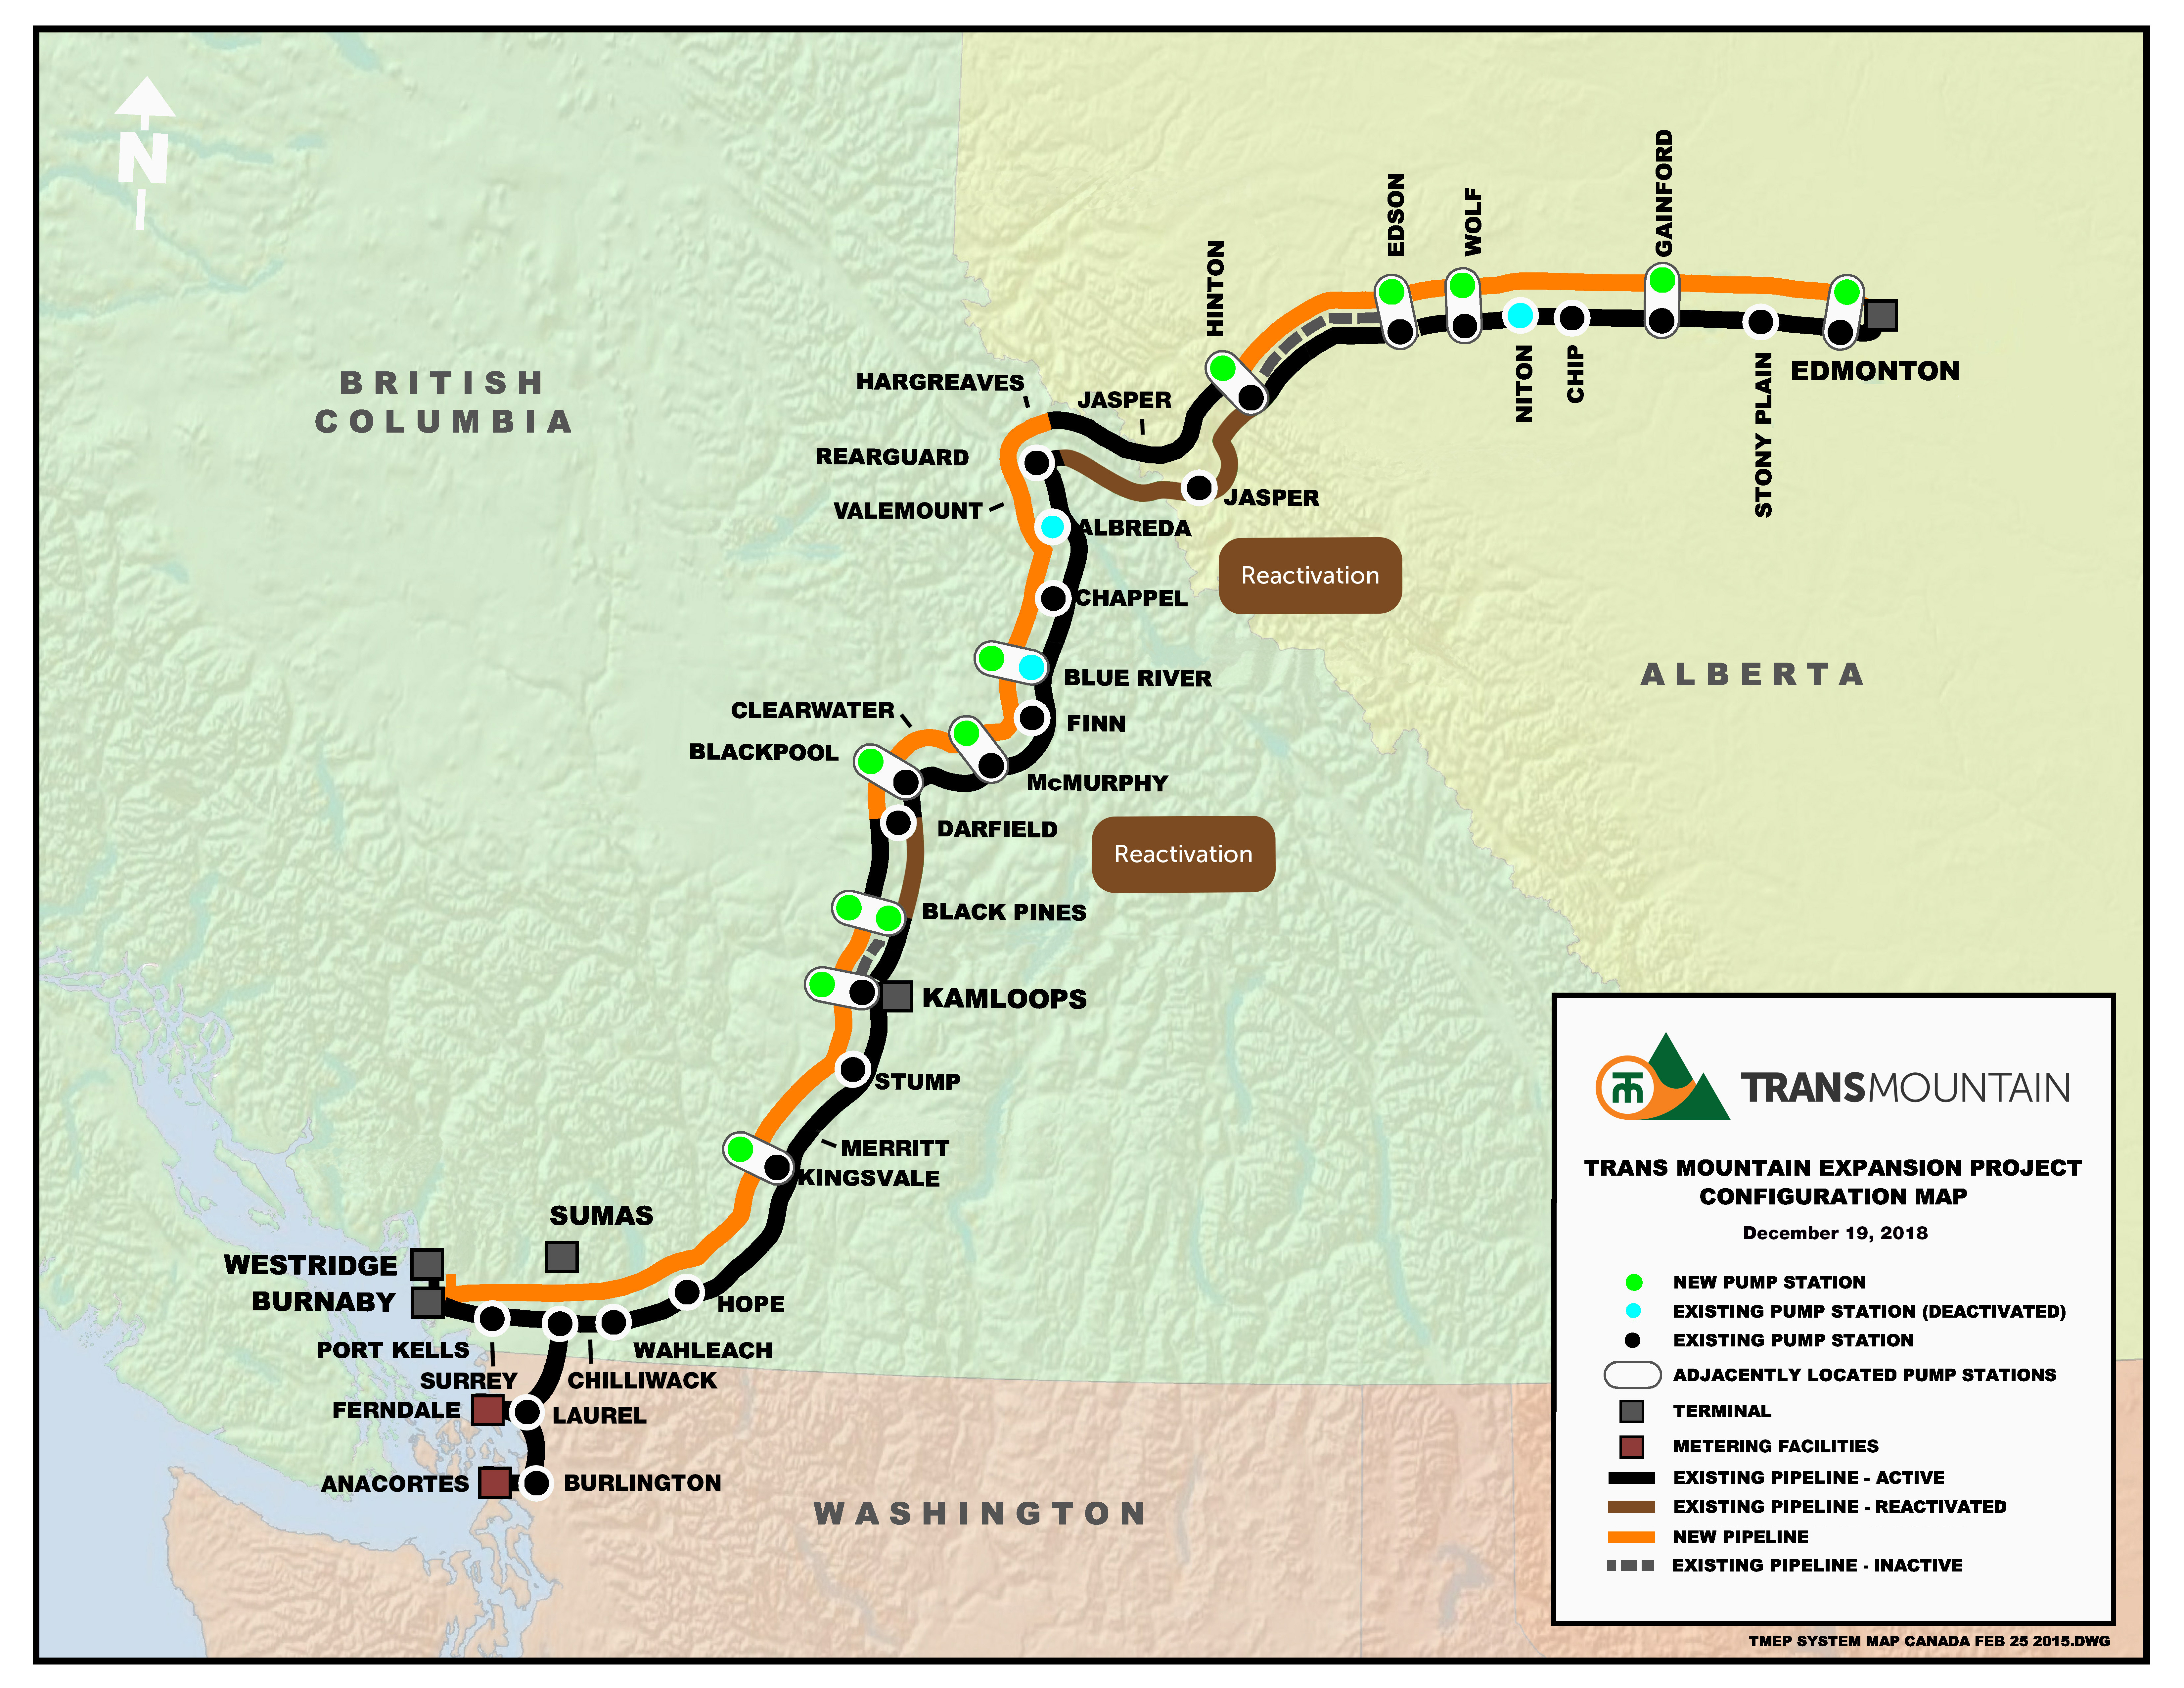
\includegraphics[width=0.67\textwidth]{Images/tmpl.jpg}
  \caption{Trans-Mountain Pipeline Expansion Project. [4]}\hrule
          \label{fig:fig2}
\end{figure}

\subsection{Report Objectives}
 This report will link incidents with reported data and bi-weekly construction reports in order to discover correlations and provide recommendations as to how data collection can be improved and how the discussed construction incidents can be limited. 
 
 All the data for analysis has been taken from the bi-weekly construction incident reports stored in the Canada Energy Regulator Database. 
% \begin{itemize}[noitemsep]
%\item g
%\item f
%\end{itemize}
%g \cite{ref1}. \newl etc. 
\subsection{Background}
The ultimate goal of the Canada Energy Regulator is to keep energy moving safely across Canada; thus our project is meant to compliment that objective through key insights found on submitted construction reports. The efforts outlined in this report that took place over the past 3 months has shown there are key issues that need to be solved, not just with safety on the workplaces, but with the submission of data format of the construction reports filings. The PDFs are all formatted in different ways, relaying extremely different structure and variables. This makes coding a single scraper to scrape these construction reports practically impossible and extremely time consuming. One of the main suggestions of this report will be to regulate the report structure; this can easily be done through online construction report submissions. This is an important aspect in improving the overall safety in the workplace; for instance, if CER is given well-formatted incident reports that are easy to retrieve information from, then it is therefore easier to analysis and find correlations among said data to create recommendations. 

\subsection{Methodology}
An overview of the tasks that have been completed (this is not necessarily an exhaustive list):
\begin{enumerate}
    \item \textit{Collect and Clean Data}, Removed redundant features from Incident Excel Data set and filled in missing locations, and;
    \item \textit{Attempt to Create PDF Scraper}, The team quickly realized this to be infeasible, decided to do it manually for the TransMountain Construction Reports, and;
    \item \textit{Conduct Analysis},  Look for correlations between incidents in order to create recommendations to improve safety in the workplace, and;
    \item \textit{Create Visualizations}, Report on findings in the form of a dashboard to create meaningful representations of the data, and;
    \item \textit{Develop Recommendations}, Final output of results, our suggestions to improve conditions and safety at CER regulated workplaces.
\end{enumerate}

\section{Data Preparation}
\subsection{Data Understanding}
 For analysis and correlations to be made, 25 PDF's and an Excel database with incident report data were referenced. Using a PDF Scraper built in R, tables were manually scraped from each incident report, that included summaries on Construction Activity, Environmental Incidents as well as Safety and Security Incidents
\subsection{Data Cleaning}
In order to clean the data from the Excel Database, features with minimal entries were removed, and filled in missing information such as "Nearest Populated Area". Many cells in the excel sheet were merged and thus required many hours to successfully unmerge all cells; this error may have been caused by the conversion to a .xlsx file from .csv.
\newline
Cleaning the PDFs was also quite an obstacle; repetitive attempts to code a universal PDF scraper that would export all the tables from various Construction Reports resulted in a realization that it was near impossible due to every PDF having considerably contrasting layouts and variables. This is discussed in detail in Section~\ref{sec:pdfscraper}.

\subsection{PDF Scraper}\label{sec:pdfscraper}

One of the project objectives that the CER is interested in is developing a process to scrape data from PDF progress reports from the pipeline construction companies. There is a wealth of data in these progress reports being held hostage by the fact that all the reports are in PDF formats. PDFs are notoriously horrible to work with structurally and thus, are a challenge to retrieve data from. 

\par The method of tackling this problem was to use open-source functional programming languages, R and Python, and various packages and libraries that can be used with them. As R is the language the team is most familiar with, the first step was to attempt to use R and any R packages that could help retrieve the data from the PDFs.

\par The team was provided with 10 recent progress report PDFs from currently active pipeline projects. Within these 10 reports, NOVA Gas Transmission Ltd submitted 5 of the 10, Enbridge Pipelines Inc. and Westcoast Energy Inc. submitted 2 each, and TransMountain submitted 1. Once the PDFs were inspected, it was noted that the progress reports had very different formats from company to company. This would prove to be one of the challenges of this task. However, PDF formats tend to stay similar within a company. Since NOVA Gas made up the majority of the PDFs that were provided, it was decided to develop a general process that functioned to scrape data from all the NOVA Gas reports. 

\subsubsection{PDF Formatting}
As previously mentioned, PDFs are difficult to extract information from in general. Using R and various packages geared towards handling PDFs can make it less painful and in some cases, these technologies actually work fairly well. However, these are usually in the case that the PDF is formatted and set-up in such a way that the designer of the PDF make it so that extracting data will be easily accessible by these PDF extraction technologies. \par While attempting to scrape the data from the provided PDFs, the team encountered many obstacles that were attributable to the formatting of the progress reports. Some of the formatting issues actually made it impossible for the team to gather any information at all. Take for example, the TransMountain progress report that was provided. This report contained some extremely poorly formatted tables, such that when attempting to extract information from it, nothing was found at all through the extraction technologies being used. See Section \ref{sec:dashboard} for some particularly poorly formatted tables from this progress report in particular.

\subsubsection{PDF Data Extraction}
To extract data from the PDFs, a process was built using R that particularly leans on the R package \textbf{tabulizer}. This package provides R bindings to the Tabula java library, which can be used to computationally extract tables from PDF documents. The Tabula technology isn't perfect and still was unable to extract from most of the PDFs that were provided for this project, but compared to all other techniques that were attempted to extract tabular information from the progress reports, it was by far the best. \par After using functions from {tabulizer} to extract the raw tables from a PDF file, the process developed takes these tables and attempts to format and structure them as best possible. Finally, the process writes the extracted and structured tables to a spreadsheet workbook.


\section{Analysis and Visualisations}\label{sec:analysis}

\begin{figure}[t]
\centering
    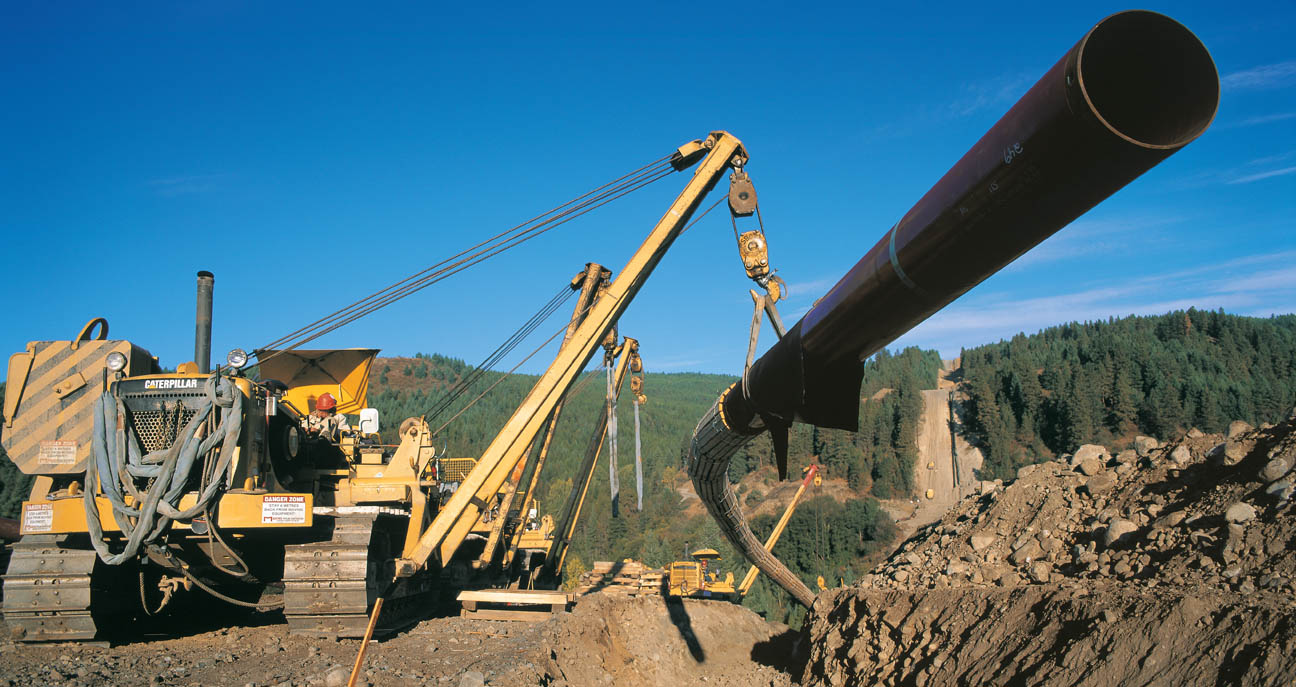
\includegraphics[width=0.67\textwidth]{Images/construction.jpg}
  \caption[Behold, the logo.]{A transmission pipeline in the process of being built. [5]}\hrule
          \label{fig:fig3}
\end{figure}

\subsection{Dashboard}\label{sec:dashboard}

One of the project objective was to design a dashboard that communicates the incident data, specifically regarding the TransMountain pipeline, as this pipeline is currently the biggest pipeline project in Canada right now. The idea for this dashboard was to provide a full report containing the incident data provided to the team by the CER, as well as including the data gathered from scraping TransMountain reports. However, as discussed in Section~\ref{sec:pdfscraper}, the TransMountain PDF format proved especially difficult to work with. The way the data and information was presented in the tables in the reports were completely incohesive with any sort of reporting without major data cleaning and processing by hand.

\par For example, in the table from page 8 of the 10/07/19 TransMountain progress report, shown in Figure~\ref{fig:badtable1}, there are \textit{table subtitles} that split the table, but aren't actually contained within the table itself. These make this data hard to communicate within a dashboard because there is no identifying column for the different project work areas. 

\begin{figure}[htbp]
\hrule\par\medskip \centering
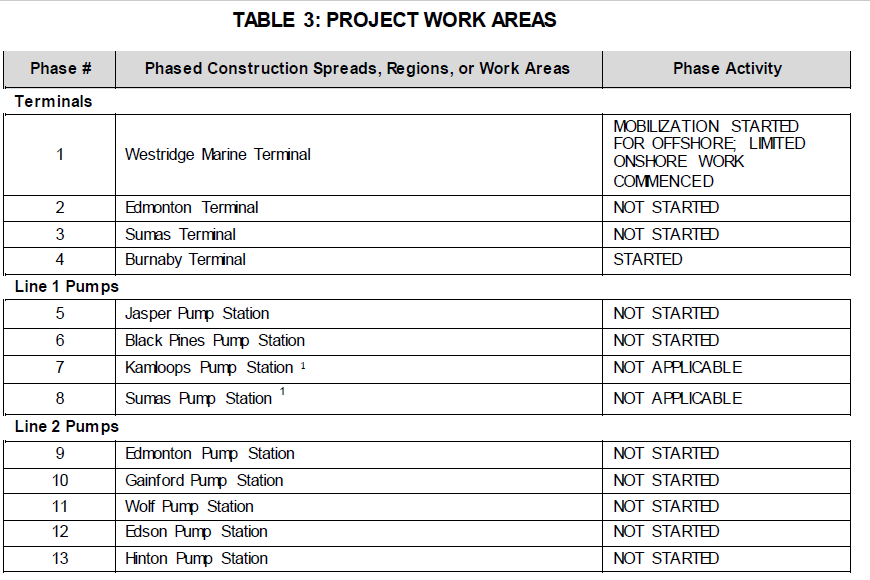
\includegraphics[width=0.8\textwidth]{Deliverables/Images/badTMtable1.PNG}
\caption[Poorly formatted table 1]{A poorly formatted table from the TransMountain reports.}
\label{fig:badtable1}
\end{figure}

\par Another example of how the TransMountain PDFs are the \textbf{worst} can be seen in Figure \ref{fig:badtable2}. This table is from page 10 of the TransMountain report. This table is bad for reporting and has many issues that would need to be corrected by hand or a tedious process, but the biggest one is the fact that it should be transposed for any sort of reporting to be done. 

\par The TransMountain reports are filled with tables like these; they all have various quirks that make them incredibly difficult to work with, especially in any reporting context. Thus, for a dashboard to be put together properly using PDF data, these issues would first need to be resolved.

\begin{figure}[htbp]
\hrule\par\medskip \centering
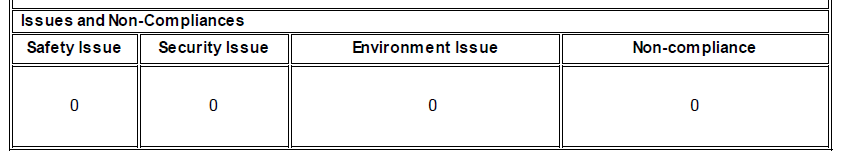
\includegraphics[width=0.8\textwidth]{Deliverables/Images/badTMtable2.PNG}
\caption[Poorly formatted table 2]{A poorly formatted table from the TransMountain reports.}
\label{fig:badtable2}
\end{figure}

\par Thus, a dashboard containing an overview of all the incidents of the TransMountain project was constructed (see Figure ~\ref{fig:dashboard1}. The data is current until the end of April 2019, per the data provided. The dashboard was constructed to give an overview of the incidents, providing high-level information, without delving too much into the details of each incident. The dashboard would be easily updated when fed new data, and because of its high-level nature, would reflect any extreme changes immediately. For example, a spike in incidents involving a release of substance would appear obvious, given the design. The dashboard was built in \textbf{PowerBI}, and is therefore interactive. This also makes it easy to inspect and identify data of interest. 

\begin{figure}[htbp]
\hrule\par\medskip \centering
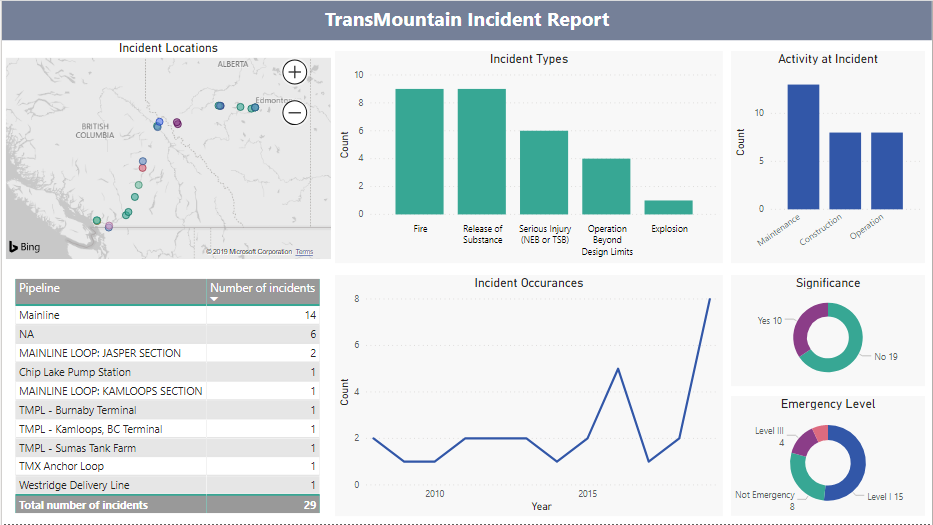
\includegraphics[width=1\textwidth]{Deliverables/Images/TransMountain_Dashboard.PNG}
\caption[TransMountain Dashboard]{Dashboard designed for incidents on the TransMountain pipeline project}
\label{fig:dashboard1}
\end{figure}

\subsection{Data Visualisation}\label{sec:visual}
\par The goal was to provide detailed information about pipeline incidents. Users can access actual pipeline data including information on all pipeline incidents in Canada, what substances were released, which province the incidents took place, and which companies were involved.

\begin{figure}[htbp]
\par The bar chart below (See figure \ref{fig:byProvince}) illustrates the location of pipeline incidents by Province. It can be seen that Alberta has the most incidents at 440 and the Northwest Territories has the least at 8. The majority of incidents took place in Alberta, British Columbia, and Ontario. Overall it can be seen that the provinces with the most major pipelines have the most accidents. 
\hrule\par\medskip \centering
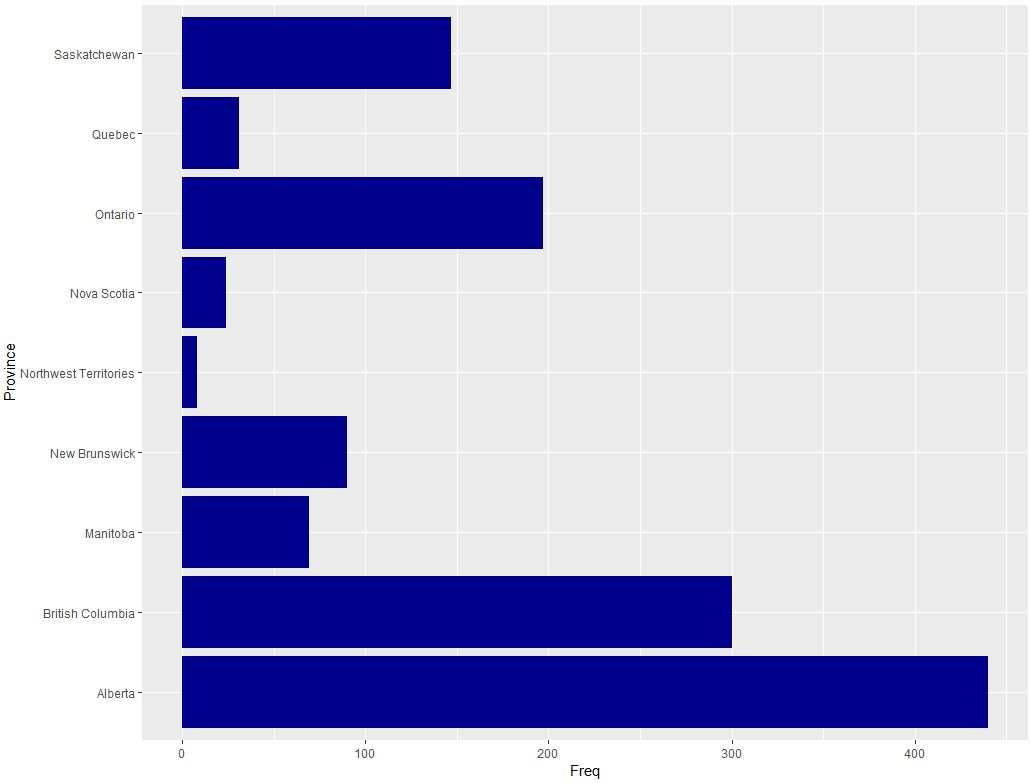
\includegraphics[width=1\textwidth]{Deliverables/Images/byProvince.JPG}
\caption[Incidents by Province]{Incidents by Province}
\label{fig:byProvince}
\end{figure}


\begin{figure}[htbp]
\par The bar chart below illustrates (See figure \ref{fig:byInc}) the distribution of incident types. As it can be seen, 669 incidents released a substance, 6 incidents ended with fatalities, and 49 incidents with serious injuries. Majority of incidents either release a substance or cause a fire. 
\hrule\par\medskip \centering
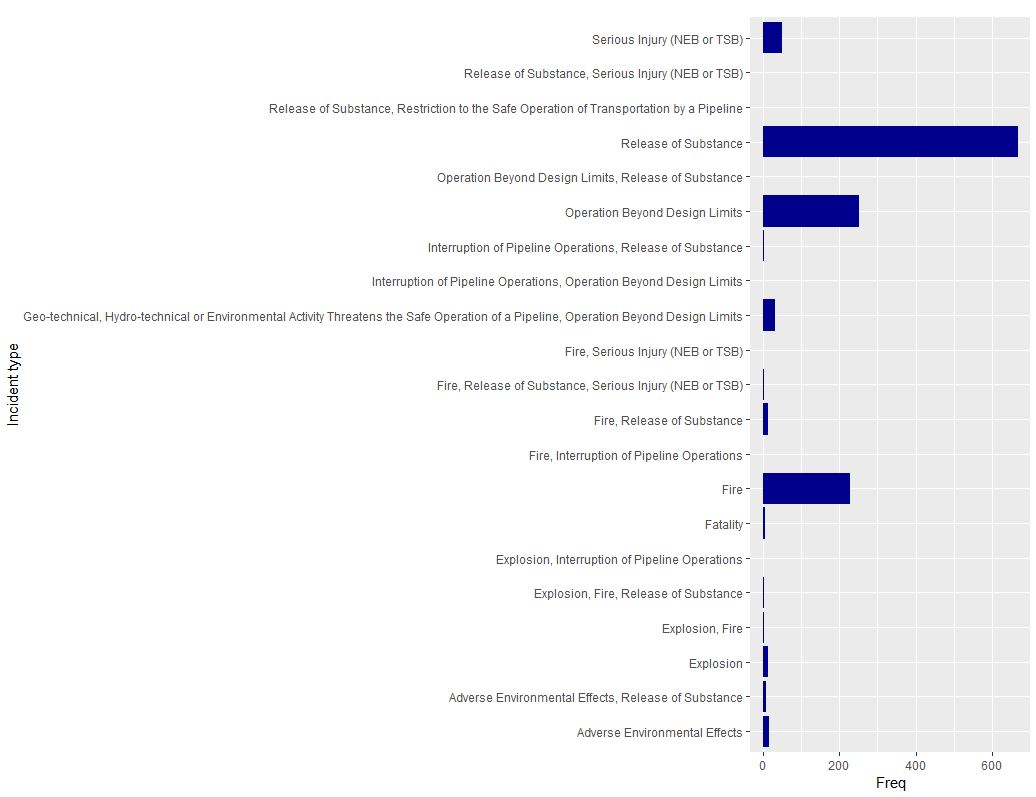
\includegraphics[width=1\textwidth]{Deliverables/Images/byIncidentType.JPG}
\caption[Incident Type]{Incident Type}
\label{fig:byInc}
\end{figure}


\begin{figure}[htbp]
\par The bar chart below illustrates (See figure \ref{fig:byWhat}) what happened during the incident. In particular, it shows the cause of the problem. It can clearly be seen that equipment failure is the leading cause followed by external interference, and then corrosion and cracking. 
\hrule\par\medskip \centering
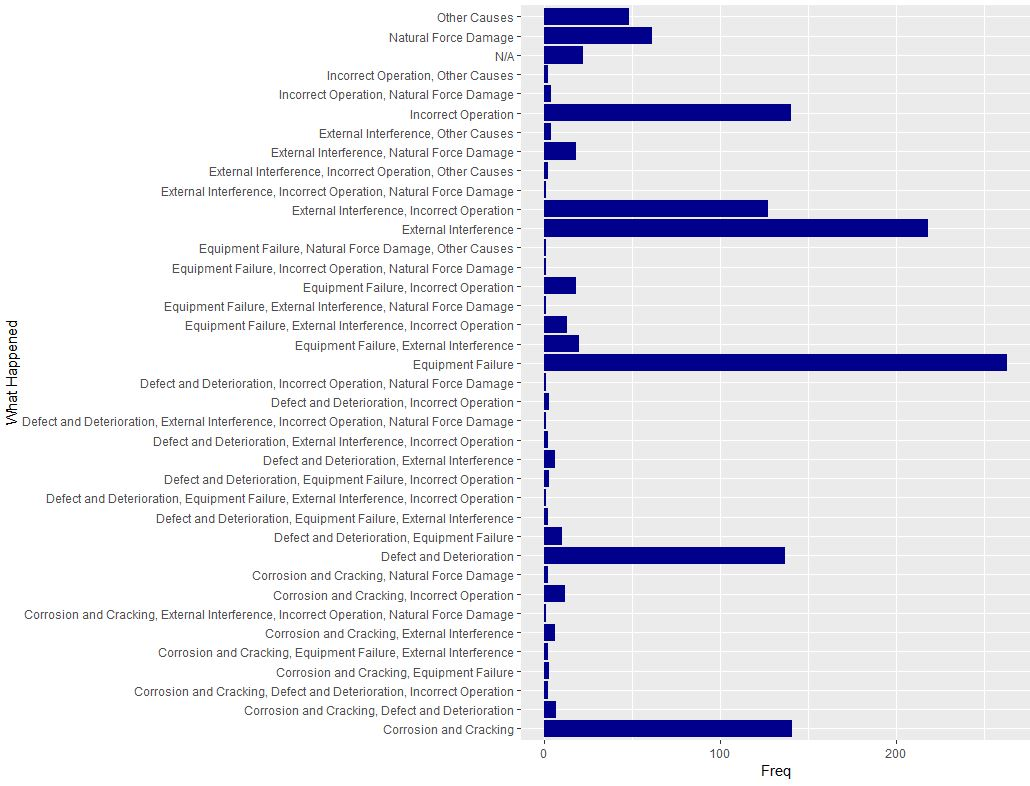
\includegraphics[width=1\textwidth]{Deliverables/Images/byWhatHappened.JPG}
\caption[What Happened]{What Happened}
\label{fig:byWhat}
\end{figure}


\begin{figure}[htbp]
\par The bar chart below (See figure \ref{fig:byCompany}) clearly illustrates that most of the incidents happened under Enbridge Pipelines. The other companies are drastically lower in comparison. 
\hrule\par\medskip \centering
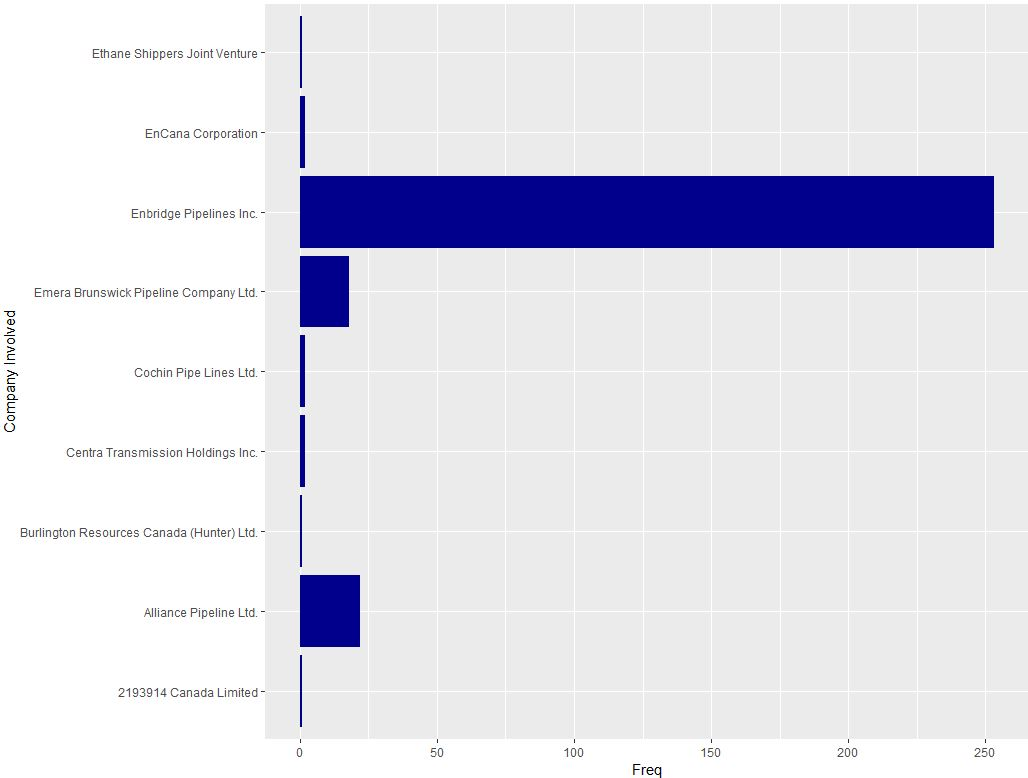
\includegraphics[width=1\textwidth]{Deliverables/Images/byCompany.JPG}
\caption[Incidents by Company]{Incidents by Company}
\label{fig:byCompany}
\end{figure}


\begin{figure}[htbp]
\par The bar chart below (See figure \ref{fig:bySubstanceR}) clearly illustrates that most incidents do not release any substance. That may be due to them ending in a fire or an explosion, or the operation being beyond design limits. But the most common substance released is sweet natural gas followed by sour natural gas. 
\hrule\par\medskip \centering
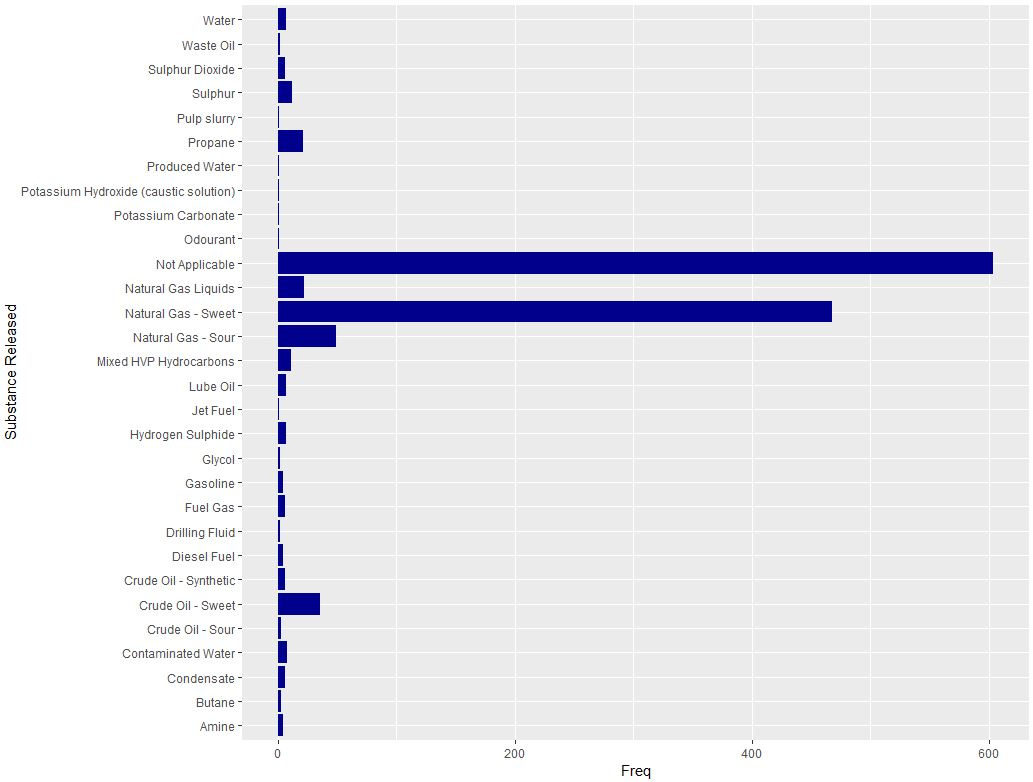
\includegraphics[width=1\textwidth]{Deliverables/Images/bySubstanceReleased.JPG}
\caption[Substance Released]{Substance Released}
\label{fig:bySubstanceR}
\end{figure}


\section{Results}
\subsection{Conclusion}
Through the process of manually cleaning and processing collected data in Excel and constructing a hard-coded PDF scraper for specific incident reports of PDF format, many conclusions can be made about the correlation between incidents as well as the data collection of construction incident reports. In terms of incidents themselves, the majority of incidents occurred on the Mainline pipeline (14/29 incidents), while maintenance was being done on a pipeline, and involved either fire or release of substances. Furthermore, there was a spike in incidents passed 2016, which may have correlation to either more documentation of incidents, or to a higher usage rate of pipelines. In terms of data collection, if the process of data collection is more direct and uniform, through the use of standardised incident report throughout companies, the overall ability to analyze and improve construction incidents can be vastly improved. A PDF Scraper can thus be uniformly used throughout each companies reports and the process of pulling tables for analysis can be made more efficient. In conclusion, through the data that was provide, a conclusion cannot be made on how construction incidents can be further prevented, however with standardized data collection further correlations can be made and implemented to prevent future construction incidents.
\subsection{Recommendations and Next Steps}
\subsubsection*{Recommendations for Data Collection}
Some of what the CER hopes to accomplish with the PDF data is infeasible given the way the data is collected and formatted. With decent data structure, the progress reports could be a powerful information source for analysis. To obtain better  data structure, assuming that progress report must be submitted in PDF format, this team recommends implementing the following across all regulated companies:
\begin{itemize}
    \item The CER create and distribute to all reporting companies a standardized progress report template, containing tables where the desired information and data can be completed by the reporting company in a structured way.
    \item Ensure that tables in reports do not span multiple pages.
    \item Ensure there is no more than 1 table per page of a given report.
    \item Attempt to include table title information within the table structure.
    \item Minimize the number of blank cells within tables.
    \item For optimal reporting, attempt to follow tidy data principals:
    \begin{itemize}[noitemsep]
        \item Each variable has its own column,
        \item Each observation has its own row,
        \item Each value has its own cell.
    \end{itemize}
\end{itemize}
%%%%%%%%%%%%%%%%%%%%%%%%
% REFERENCES %%%%%%%%%%%
%%%%%%%%%%%%%%%%%%%%%%%%
\begin{thebibliography}{99}
\bibitem{ref1} Leeper, T., Paskhalis, T. rOpenSci: The tabulizer package, {\it rOpenSci}. (https://docs.ropensci.org/tabulizer/)

\bibitem{ref2} Boily, P., Pelletier, M. [2019], Dashboards and Data Visualization, with Examples, {\it Data Action Lab}. (https://www.data-action-lab.com/2019/09/16/dashboards-and-data-visualization-with-examples/)

\bibitem{ref3} Wickham, H. [2014], Tidy Data, {\it Journal of Statistical Software}. doi: 10.18637/jss.v059.i10

\bibitem{ref4} Planning the Route. (n.d.). Retrieved from https://www.transmountain.com/planning-the-route.

\bibitem{ref5} Construction. (n.d.). Retrieved from https://www.aboutpipelines.com/en/pipeline-101/construction/.

\end{thebibliography}

\end{document}
